\documentclass{endm}
\usepackage{endmmacro}
\usepackage{graphicx}
\usepackage{float}
\usepackage[utf8]{inputenc}
\usepackage[spanish,activeacute]{babel}
\usepackage{setspace}  
\setlength{\textwidth}{150mm}

% The following is enclosed to allow easy detection of differences in
% ascii coding.
% Upper-case    A B C D E F G H I J K L M N O P Q R S T U V W X Y Z
% Lower-case    a b c d e f g h i j k l m n o p q r s t u v w x y z
% Digits        0 1 2 3 4 5 6 7 8 9
% Exclamation   !           Double quote "          Hash (number) #
% Dollar        $           Percent      %          Ampersand     &
% Acute accent  '           Left paren   (          Right paren   )
% Asterisk      *           Plus         +          Comma         ,
% Minus         -           Point        .          Solidus       /
% Colon         :           Semicolon    ;          Less than     <
% Equals        =           Greater than >          Question mark ?
% At            @           Left bracket [          Backslash     \
% Right bracket ]           Circumflex   ^          Underscore    _
% Grave accent  `           Left brace   {          Vertical bar  |
% Right brace   }           Tilde        ~

\newcommand{\Nat}{{\mathbb N}}
\newcommand{\Real}{{\mathbb R}}
\begin{document}
% DO NOT REMOVE: Creates space for Elsevier logo, ScienceDirect logo
% and ENDM logo
\begin{verbatim}\end{verbatim}\vspace{.5cm}
\begin{frontmatter}
\title{Las Reglas del Congreso}
\author{Diego Santos\thanksref{sdemail}}
\author{Axel Savizky  \thanksref{raemail}}
\address{Reglas de Asociación y Simulación de Patrones - Departamento de Computación - Universidad de Buenos Aires - Bs.As., Argentina}
\thanks[raemail]{Email:
  \href{mailto:axel.savizky@gmail.com} {\texttt{\normalshape
   axel.savizky@gmail.com}}}
\thanks[sdemail]{Email:
  \href{mailto:diego.h.santos@gmail.com} {\texttt{\normalshape
   diego.h.santos@gmail.com}}}
\begin{abstract}
Todos los años durante el período de marzo a diciembre 257 diputados se reunen para determinar que nuevas leyes regirán sobre el pueblo argentino. En el presente trabajo se analizó un conjunto de votaciones de la Cámara de Diputados de la Nación con el fin de identificar las reglas que se esconden en las sanciones de leyes.
\end{abstract}
\begin{keyword}
Diputados, Transacciones, Monotonía, Leyes, Ausencias.
\end{keyword}
\end{frontmatter}
\section{Presentación}\label{intro}
El objetivo del trabajo es determinar reglas en las votaciones de ley de la Cámara de Diputados del Congreso de la Nación Argentina a partir de los resultados de las votaciones de cada ley correspondientes al período de marzo a septiembre de 2018.\\

Durante este período se trataron 72 leyes, involucrando a cada una 257 diputados de 32 partidos poltíticos agrupados en 17 interbloques.\\

La datos para la confección del reporte se obtuvieron de la página web de la Cámara de Diputados. \footnote{https://www.diputados.gov.ar/}

\subsection{Set de Datos}

El set de datos utilizado consta de 72 archivos csv donde en cada uno de ellos se muestra por fila: \\

Diputado $|$ Partido $|$ Provincia $|$ ¿Cómo voto?\\

Es decir que cada archivo tiene 257 filas donde en cada una se presenta un diputado, el partido al que pertenece, la provincia a la que representa y cual fue su voto.\\

El campo ¿Cómo voto? tiene 5 estados posibles:\\

\begin{itemize}
\item Presidente: Si ejerció como presidente de la sesión.
\item Afirmativo: Si su voto a favor de la sanción de la ley.
\item Negativo: Si su voto fue en contra de la sanción de la ley.
\item Abstención: Si se excuso de votar.
\item Ausente: Si no estuvo presente en el recinto.
\end{itemize}

\subsection{Transacción}

Los datos en el formato que se obtuvieron no resultan útiles para establecer reglas más allá de las evidentes, por lo que fue necesario reagrupar los datos en otro tipo de transacción. \\

De un análisis de los datos en crudo se descubrió que en casi la totalidad de los casos la votación de los diputados es en bloque. Es decir, siguen una disciplina partidaria donde todos los pertenecientes al mismo partido votan igual, sin importar la provincia a la que pertenezcan. Además dicha disciplina suele aplicarse también para los interbloques. \\

Entonces el voto de un diputado esta condicionado a la decisión del partido y no esta condicionado por la provincia a la que representa. Entonces para el armado de la transacción se consideró que no es necesario contar con el nombre del diputado, sino por como voto su partido esa ley. \\

Además como cada provincia esta representada por un subconjunto de diputados, proporcional a la población de dicha provincia, que pertenecen a un subconjunto de los partidos, se determino que una forma conveniente de representar la decisión de la provincia es tomando el valor de la mayoría de los votos de los diputados que la representan. \\

En base a esto se decidió construir la transacción con el siguiente formato: \\

Ley $|$ Estado $|$ Partido1 $|$...$|$ Partido32 $|$ Provincia1 $|$ ... $|$ Provincia22 \\

Donde el valor de cada campo columna puede tomar los siguientes valores: \\

Para \textbf{Ley} \\

El nombre de archivo csv que corresponde al dataset de un tratamiento de ley. \\

Para \textbf{Estado} \\

\begin{itemize}
\item $LEY APROBADA$: Si la ley fue aprobada.
\item $LEY RECHAZADA$: Si la ley no fue aprobada. \\
\end{itemize}

 Para \textbf{Partido X} \\

\begin{itemize}
\item $PARTIDO [AFIRMATIVO]$
\item $PARTIDO [NEGATIVO]$
\item $PARTIDO [ABSTENCION]$
\item $PARTIDO [AUSENTE]$ 
\item $PARTIDO [EMPATE]$ \\
\end{itemize}

Donde el valor se define siguiendo el criterio de las mayorías. Para la ley que presenta la transacción se contabilizan los votos de todos los diputados del partido
y se asigna el resultado de la mayoria. EMPATE se utiliza si no hay un criterio mayoritario. \\

Por ejemplo: \\

Partido1 que tiene 5 diputados representantes, 4 votan afirmativo y 1 ausente, al haber mas votos positivos el resultado es PARTIDO1 [AFIRMATIVO] \\

Partido2 que tiene 2 diputados representantes, 1 vota afirmativo y otro 1 ausente. El resultado es PARTIDO1[EMPATE] \\

Para \textbf{Provincia X} \\

\begin{itemize}
\item $PROVINCIA [AFIRMATIVO]$
\item $PROVINCIA [NEGATIVO]$
\item $PROVINCIA [ABSTENCION]$
\item $PROVINCIA [AUSENTE]$ 
\item $PROVINCIA [EMPATE]$ \\
\end{itemize}

Donde el valor se define siguiendo el criterio de las mayorías. Para la ley que presenta la transacción se contabilizan los votos de todos los diputados que pertenecen a esa provincia, sin considerar el partido y se asigna el resultado de la mayoria. EMPATE se utiliza si no hay un criterio mayoritario. \\

Por ejemplo: \\

Una provincia que tiene 2 partidos que la representan en el recinto. El Partido1 tiene 5 diputados, 4 votan afirmativo y 1 ausente. El Partido2 tiene 3 diputados que votan de forma negativa. El resultado es PARTIDO1 [AFIRMATIVO]. \\

Esta representación de transacción permite clusterizar los datos individuales de cada diputado evitando la redundancia de datos permitiendo obtener reglas generalizadas sobre los partidos y los interbloques a los que pertenecen. \\

El motivo por el que las ausencias son consideradas en el armado de la transacción es que la presencia o no de un bloque en ciertos casos puede ser parte del armado de una estrategia legislativa, especialmente en los partidos que no son un monobloque.

\section{Reglas}\label{desarrollo}

Para encontrar las reglas que determinan el comportamiento del set de transacciones se utilizó la implementación del algoritmo $Apriori$ del paquete aRules del lenguaje de programación $R$.\\

El objetivo es a partir de las reglas encontradas, describir el comportamiento que lleva a que una ley sea aprobada o rechazada, para facilitar la descripción se analizan por separado las reglas por separado para luego sobre el fin del trabajo, para luego sobre el fin del trabajo establecer las reglas sobre la sanción o rechazo de la ley.\\

De las reglas obtenidas se presenta un análisis de algunas de las más relevantes para describir la dinámica de la Cámara Baja. 

En la sección de $Diputados$ se describen las reglas que siguen los diputados en relación al partido que pertenecen.\\

En la sección de $Partidos$ se describen las reglas que relacionan a un partido con otro. Es decir que partidos votan frecuentemente de la misma forma o de forma opuesta.\\

En la sección de $Interbloques$ se describen las reglas que relacionan a los partidos del mismo interbloque y luego las del interbloque en conjunto contra los demás partidos.\\

En la sección de $Provincias$ se describen las reglas que relacionan a las provincias entre sí.\\

En la sección de $Partidos y Provincias$ se describen las reglas que relacionan a los partidos con las provincias.\\

En la sección de $Sanciones de Ley$ se describen las reglas son las que llevan a la aprobación o rechazo de una ley.\\

Para una mejor visualización e interpretación de las reglas es conveniente intercalar la lectura de esta sección con la infografía de leyes detallada en el archivo \textbf{$infografia_leyes.html$} la cual permite explorar la totalidad de las reglas de las secciones antes mencionadas. Dentro de la carpeta \textbf{$reglas XML$} se encuentran en formato xml un conjunto de archivos que contienen todas las reglas obtenidas para cada sección.\\

Para una mayor simplicidad de análisis en cada una de las secciones de estudio se limito el dataset a los items a estudiar en cada sección. El objetivo fue procesar menos datos para obtener resultados enfocados al estudio de la sección, además de una mayor simplicidad en el script que genera las reglas.\\

Como parametros del algoritmo apriori se asigna confidence = 0.80, pues interesa encontrar patrones muy frecuentes. El valor del soporte será estudiado para cada sección dependiendo del dataset. \\

Los dataset puede encontrarse en la seccion /datos. En el Apéndice se detalla cada uno de ellos. \\

\subsection{Diputados}

Del análisis exploratorio de los datos en crudo se pudo observar y determinar que un diputado perteneciente a un partido cualquiera vota de la misma forma que el resto de sus compañeros de partido. Este comportamiento se repite en 71 de las 72 sesiones analizadas.\\

Sin importar la provincia a la que represente, un diputado vota alineado al partido al que pertenece.\\

\subsection{Partidos}

En esta sección se presentan las reglas que involucran a los partidos. La intención es establecer reglas que permitan inferir que partidos votan alineados y quienes lo hacen de forma opuesta. \\

El dataset utilizado es transaccionespartidos.csv. Se analiza la distribución de los datos para encontrar un valor para el soporte del algoritmo apriori. \\

\begin{center}
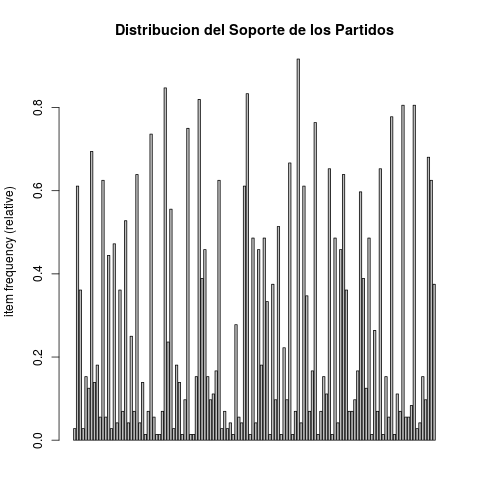
\includegraphics[scale=0.4]{graficos/soportesPartidos.png}
\end{center}  \\

Debido a la gran cantidad de datos para esta sección el parámetro de confianza para el algoritmo de apriori será de 0.90 y el soporte de 0.60. \\

Se obtuvieron 42 reglas que pueden encontrarse en el archivo reglasPartidos.xml.  \\

Se considerán destacables las siguientes reglas respecto al partido oficialista: \\

{Coalicion Civica[NEGATIVO]} \Longrightarrow {PRO[NEGATIVO]}

\\ Con un soporte de 0.61, confianza 1 y lift 1.5.\\

{Partido por la Justicia Social[NEGATIVO]} \Longrightarrow {PRO[NEGATIVO]} \\

Con un soporte de 0.61, confianza 1 y lift 1.5.\\

{Union Civica Radical[NEGATIVO]}  \Longrightarrow {PRO[NEGATIVO]}\\

Con un soporte de 0.62, confianza 1 y lift 1.5.\\

Al darse el voto negativo de estos partidos es esperable que también el PRO vote de la misma forma. Cabe destacar que estos partidos se encuentran dentro del mismo interbloque, por lo que es esperable que sus votos estén en síntonia. \\

{PRO[NEGATIVO]}  \Longrightarrow {Frente para la Victoria - PJ[POSITIVO]} \\

Con un soporte de 0.61, confianza de  0.95 y lift 1.16. Es esperado que el voto del Frente para la Victoria - PJ sea opuesto al del PRO, confirmando la coyuntura política del país. \\ 

También son destacables las reglas sobre los partidos que pueden englobarse dentro del denominado $Peronismo$ \\

{Justicialista por Tucuman[POSITIVO]} \Longrightarrow {Justicialista[POSITIVO]} \\

Con un soporte de  0.61, confianza 1 y lift 1.2\\


{Peronismo para la Victoria[POSITIVO]} \Longrightarrow {Frente para la Victoria - PJ[POSITIVO]}  \\

Con un soporte de 0.61, confianza 0.93y lift 1.14\\

{Unidad Justicialista[POSITIVO]}  \Longrightarrow {Justicialista[POSITIVO]} \\

Con un soporte de 0.62, confianza 0.91 y lift 1.10\\

{Frente para la Victoria - PJ[POSITIVO]}    \Longrightarrow {Federal Unidos por una Nueva Argentina[POSITIVO]}\\

Con un soporte de 0.76, confianza 0.93 y lift 1.10\\

Puede verse que hay una gran correlación entre sus votos, que luego más adelante podrá ser confirmado analizando el voto de los interbloques.\\

Una regla que resultó ser inesperada es \\

{Fte. de Izquierda y de los Trabajadores[POSITIVO]} \Longrightarrow {Frente para la Victoria - PJ[POSITIVO]}\\

Con un soporte de 0.61, confianza 0.97 y lift 1.1. A priori no era esperada tanta correlación entre el principal partido de izquierda y el FPV. \\


\subsection{Interbloques}

En esta sección se presentan las reglas que representan el comportamiento de los partidos agrupados en Interbloques.\\

El dataset utilizado para las reglas entre los miembros del interbloque contiene todos los votos de los partidos pertenecientes al interbloque. La longitud de las reglas pedidas al algoritmo son del tamaño del bloque, a fin de obtener del lado izquierdo todos los partidos menos uno, que estará del lado derecho.\\

El dataset utilizado para las reglas entre el interbloque con los demás partidos contiene todos los votos de todos los partidos. En el algoritmo apriori se indico que se generen las reglas con todo el interbloque del lado izquierdo quedando del lado derecho un partido que no pertenece al interbloque. \\

\textbf{Interbloque Cambiemos}\\

\textit{Dentro del Interbloque} \\

El dataset utilizado es transaccionescambiemos.csv. Se analiza la distribución de los datos para encontrar un valor para el soporte del algoritmo apriori. \\

\begin{center}
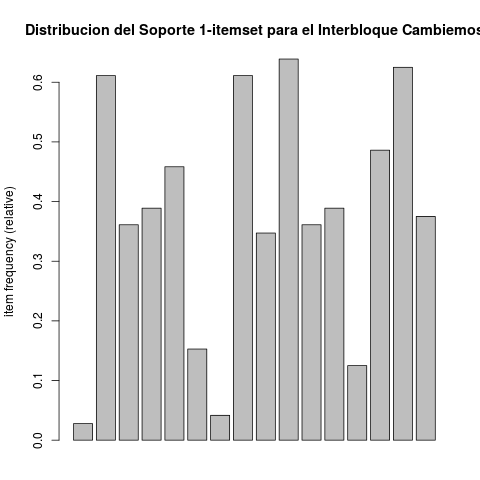
\includegraphics[scale=0.4]{graficos/soportesCambiemos.png}
\end{center}

En base a la distribución de los datos observada un valor adecuado para el soporte es 0.1. \\

Con esta configuración y luego de eliminar las reglas redundantes se obtuvieron 4 reglas. Se encuentran en el archivo reglasCambiemos.xml  \\

\begin{center}
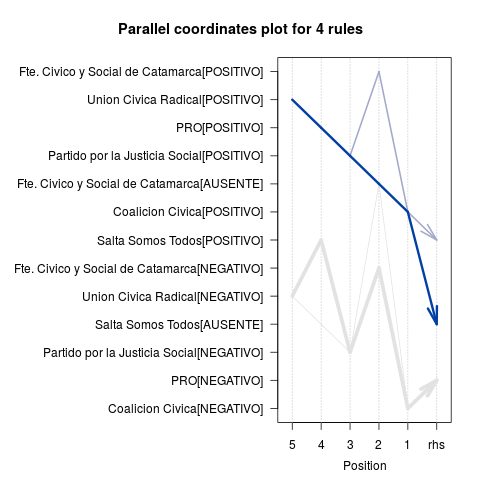
\includegraphics[scale=0.4]{graficos/paracoordInterbloquesCambiemos.png} \\
\scriptsize{Figura: La forma en que voto un partido se representa sobre el eje y. Mientras que la intersección sobre  los números representa que se encuentra del lado izquierdo y la flecha representa cual valor se ubica en el lado derecho.}
\end{center}

Se considerán destacables las reglas: \\

{Coalicion Civica[POSITIVO],
 Fte. Civico y Social de Catamarca[POSITIVO],
 Partido por la Justicia Social[POSITIVO],   
 PRO[POSITIVO],        
 Union Civica Radical[POSITIVO]} \Longrightarrow{Salta Somos Todos[POSITIVO]} \\

Con soporte de 0.15, confianza de 1 y lift de 2.05. Muestra  con un soporte de 0.15 que el interbloque vota en conjunto de forma positiva. \\

{Coalicion Civica[NEGATIVO],         
Fte. Civico y Social de Catamarca[NEGATIVO],
Partido por la Justicia Social[NEGATIVO],
Salta Somos Todos[POSITIVO],
Union Civica Radical[NEGATIVO]}  \Longrightarrow {PRO[NEGATIVO]} \\

Con soporte de 0.26, confianza de 1 y lift de 1.56. Muestra  con un soporte de 0.15 que no vota unido de forma negativa. Sino que el partido Salta Somos Todos suele mostrarse autónomo. \\

Una curiosidad esta dada por la siguiente regla

{Coalicion Civica[POSITIVO],                    
Fte. Civico y Social de Catamarca[AUSENTE], 
Partido por la Justicia Social[POSITIVO], 
PRO[POSITIVO], 
Union Civica Radical[POSITIVO]}             \Longrightarrow  {Salta Somos Todos[AUSENTE]} \\

Con soporte de 0.19, confianza de 1 y lift de 2.57. Muestra que los miembros de los partidos Salta Somos Todos y Fte. Civico y Social de Catamarca suelen ausentarse juntos cuando los demás miembros votan de forma positiva. \\


\textit{Interbloque contra el resto de los partidos} \\

El dataset utilizado es transaccionespartidos.csv. Se analiza la distribución de los datos para encontrar un valor para el soporte del algoritmo apriori. \\

\begin{center}
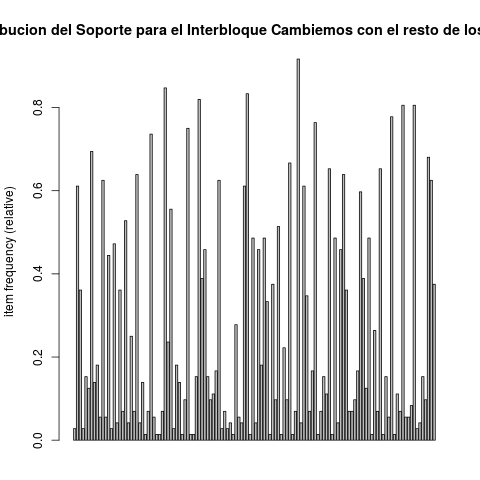
\includegraphics[scale=0.4]{graficos/soportesCambiemosRestoPartidos.png}
\end{center}

En base a la distribución de los datos observada un valor adecuado para el soporte es 0.25. \\

Con esta configuración y luego de eliminar las reglas redundantes se obtuvieron 9 reglas. Se encuentran en el archivo reglasCambiemosRestoPartidos.xml  \\

\begin{center}
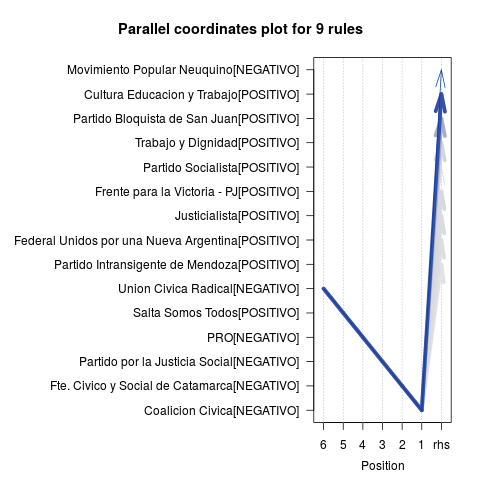
\includegraphics[scale=0.4]{graficos/paracoordCambiemosRestoPartidos.png} \\
\scriptsize{Figura: La forma en que voto un partido se representa sobre el eje y. Mientras que la intersección sobre  los números representa que se encuentra del lado izquierdo y la flecha representa cual valor se ubica en el lado derecho.}
\end{center} \\

Se considerán destacables las reglas: \\

{Coalicion Civic[NEGATIVO],    
Fte. Civico y Social de CatamarcaNEGATIVO],     
Partido por la Justicia Social[NEGATIVO],
PRO[NEGATIVO],      
Salta Somos Todos[POSITIVO],
Union Civica Radical[NEGATIVO]}              \Longrightarrow {Movimiento Popular Neuquino[NEGATIVO]} \\

Con soporte de 0.25, confianza de 0.94 y lift de 1.94. El partido Movimiento Popular Neuquino suele acompañar en el voto Negativo a la mayoria del interbloque, que vota mientras que el partido Salta Somos Todos vota de forma distinta al interbloque. \\

{Coalicion Civica[NEGATIVO],
Fte. Civico y Social de Catamarca[NEGATIVO],    
Partido por la Justicia Social[NEGATIVO],       
PRO[NEGATIVO], 
Salta Somos Todos[POSITIVO],                     
Union Civica Radical[NEGATIVO]}              \Longrightarrow {Frente para la Victoria - PJ[POSITIVO]} \\

Con soporte de 0.26, confianza de 1 y lift de 1.22. El partido Frente para la Victoria - PJ vota de forma positiva cuando el interbloque vota de forma negativa excepto Salta Somos Todos que vota positivo.\\

De las reglas obtenidas puede deducirse que el partido Salta Somos Todos suele votar en contra del interbloque cuando este lo hace de forma negativa. Y se puede inferir que suele acompañar a la oposición a su interbloque. \\

\subsection{Provincias}

\subsection{Partidos y Provincias}
\subsection{Sanciones de Ley}

\section{Conclusiones}

\section{Referencias Bibliográficas}

\end{document}
